\documentclass[11pt,a4paper]{article}
\usepackage[margin=25mm]{geometry}
\usepackage[T1]{fontenc}
\usepackage[utf8]{inputenc}
\usepackage[british]{babel}
\usepackage{lmodern,microtype,amsmath,amssymb,amsthm,booktabs,tabularx,graphicx}
\usepackage{xcolor,caption,placeins,tikz}
\usetikzlibrary{arrows.meta,positioning,calc}
\usepackage[colorlinks=true,linkcolor=teal,citecolor=teal,urlcolor=teal]{hyperref}
\captionsetup{font=small,labelfont=bf}
\setlength{\parskip}{4pt}
\setlength{\parindent}{0pt}
\setlength{\emergencystretch}{2em}
% Exactly the palette of the generated figures (tools/paper_network_figures.py),
% so drawn and generated panels are one visual language.
\definecolor{ink}{HTML}{243340}
\definecolor{pale}{HTML}{D8EEF0}
\definecolor{warm}{HTML}{C86428}
\definecolor{figteal}{HTML}{007F86}
\definecolor{figgrey}{HTML}{77818D}
\definecolor{figlight}{HTML}{F2F5F7}
\tikzset{box/.style={draw=figteal,rounded corners=3pt,fill=pale,align=center,
   inner sep=7pt,font=\sffamily\small,text=ink},
 solidbox/.style={rounded corners=3pt,fill=figteal,align=center,inner sep=7pt,
   font=\sffamily\small,text=white},
 innode/.style={circle,draw=white,line width=1.2pt,fill=pale,minimum size=8.5mm,
   inner sep=0pt,font=\sffamily\small,text=ink},
 outnode/.style={circle,draw=white,line width=1.2pt,fill=warm,minimum size=8.5mm,
   inner sep=0pt,font=\sffamily\small,text=white},
 outbox/.style={rounded corners=3pt,fill=warm,align=center,inner xsep=6pt,
   inner ysep=5pt,font=\sffamily\small,text=white},
 panel/.style={font=\sffamily\small,text=ink,anchor=south west},
 edgelab/.style={font=\sffamily\scriptsize,text=ink,inner sep=2pt},
 onecell/.style={minimum width=6.4mm,minimum height=4.5mm,inner sep=0pt,
   fill=figteal,text=white,draw=white,line width=.7pt,font=\sffamily\scriptsize},
 zerocell/.style={minimum width=6.4mm,minimum height=4.5mm,inner sep=0pt,
   fill=figlight,text=figgrey,draw=white,line width=.7pt,font=\sffamily\scriptsize},
 arrow/.style={-{Stealth},line width=1.05pt,draw=figgrey},
 cutarrow/.style={dashed,line width=1.05pt,draw=warm}}
\newtheorem{proposition}{Proposition}
\newcommand{\Maj}{\operatorname{MAJ}_3}
\newcommand{\F}{\mathbb F}
\hypersetup{pdftitle={Solutions to the challenges proposed by 0xPARC},pdfauthor={Alberto Hernandez-Espinosa}}
\title{Solutions to the challenges proposed by 0xPARC\\[5pt]
\large Exact representations, index deconvolution and constrained computation}
\author{Alberto Hernandez-Espinosa}
\date{17 September 2026}
\begin{document} 
\maketitle
\begin{abstract}

In this report I present possible solutions to five of the eight challenges
raised by 0xPARC~\cite{challenge}: the majority construction and the four
integer conditions expressed in a finite field. These are the questions one
method answers. I use an index-deconvolution method to recover a Boolean
system's functional description from its behaviour alone; run on a canonical
decision diagram it does so without enumerating states. The same method
supplies the gates for the arithmetic questions: each cell is stated as an
integer relation and whatever gate the method returns is what is compiled, so
the classical full adder is recovered rather than assumed. The remaining three
questions have answers that this method does not supply, and reporting them
here would credit it with work it did not do. Supplementary Information gives
the proofs, complete specifications and verification evidence.
\end{abstract}

\section{Disclaimer on the use of AI}
AI tools were used as assistants for constructing the testbed, searching for
and corroborating bibliography and related work, discussing the solutions
presented here, and reviewing grammar and phrasing. The ideas, research,
methods, validation, interpretations and claims are original to the author,
who takes responsibility for the final content and for independently checking
the cited sources.

\section{What index deconvolution is}
\label{sec:index-capability}

Index deconvolution is the Boolean-network component used throughout this
response. Its lineage is algorithmic information dynamics: the study of how an
integrated system responds to interventions, how a generative description
exposes behaviour, and how such descriptions support explanation and
prediction~\cite{hernandez2019aid,hernandez2021aid}. It takes information to be
program size, in the sense of Kolmogorov and
Chaitin~\cite{kolmogorov1965,chaitin1966,li2019}, rather than a distribution
over states, and it specialises that view to exact finite Boolean descriptions;
it does not compute Kolmogorov complexity itself. In practice it compresses the
behaviour of a complex Boolean network into a construction small enough to
answer the queries that matter, yet faithful enough to express the behaviour of
the system exactly. Single-bit perturbations isolate the responsive
coordinates, the restricted behaviour is matched against a canonical gate
family, and the recovered description is replayed forward, where it must
reproduce the original behaviour exactly.

The method is under active development, and a full account of it is in
preparation for publication; what is used here is the part that is settled, and
the implementation accompanies this response~\cite{causalbool}.

% Role ledger, retained here as a comment; the generated ledger and its
% definitions live in Supplementary Section S7.
% \begin{center}
% \begin{tabular}{llp{0.56\linewidth}}
% \toprule
%  & Role & What the method supplies\\\midrule
% Q2 & derives & majority recovered to 151 inputs, identical to an independent threshold\\
% Q5 & derives & the comparator the range predicate is built from\\
% Q6 & derives & the comparator and inequality cells at 254 bits\\
% Q7 & derives & the full adder and partial product the 64-bit multiplier is built from\\
% Q8 & bounds & a measurement of where the representation stops working\\
% \bottomrule
% \end{tabular}
% \end{center}

This is what decides which questions appear below. Four of them are answered by
an object the method returned, and the fifth, Q8, is not answered by it at all:
there the contribution is a measurement of why, and the answer is the direct
limb construction. Questions whose answers the method does not supply are left
to another account rather than reported here with the method attached to them.
Supplementary Sections~S7--S9 record, answer by answer, what the method
supplies, together with the evidence, the denominators and the limits.
Section~S9 in particular separates what the strongest of those measurements
does and does not establish.


\section{Constructing and recovering majority (Q2)}
A three-input majority gate returns one when at least two inputs are one.
\textit{The question asks whether these gates can compute majority on 2025 inputs,
with free duplication of wires}. \textbf{They can.} The useful identity can be
understood by temporarily allowing a more general monotone Boolean function
$f$: changing an input from zero to one never lowers its output.

Choose three distinct inputs $a,b,c$. Form three simpler functions by
replacing $b$ with $a$, $c$ with $b$, and $a$ with $c$, respectively. Then
\begin{equation}\label{eq:maj}
f=\Maj\bigl(f_{b\gets a},f_{c\gets b},f_{a\gets c}\bigr).
\end{equation}
If the three input bits agree, all substitutions preserve the assignment.
Otherwise, one preserves it, one increases a bit and one decreases a bit.
Their outputs therefore bracket the original output, with the original
itself among them. Their majority equals $f$.

Each substitution removes an active input. Odd majority is also self-dual:
complementing every input complements the output. Both properties survive
substitution, and a monotone self-dual function on at most two inputs is
just an input wire. Repeating Eq.~\eqref{eq:maj} therefore produces a circuit
containing only three-input majority gates. The proof applies to every odd
input count, including 2025. It gives existence; its loose size bound does
not establish an economical circuit at that scale.

\subsection{A network we can inspect completely}
For five inputs, the construction emits the seven gates in
Figure~\ref{fig:network}. Each arrow carries an input bit or the output of
an earlier gate. For example, $g_0=\Maj(x_0,x_2,x_4)$ and
$g_1=\Maj(x_0,g_0,x_3)$. The final gate takes $g_1,g_3,g_5$.
Reading across a row of the connection matrix identifies the three sources
of that gate; evaluating the gates in order gives the output.

Take input $11100$, written in the order $x_0,\ldots,x_4$. Its first three
bits are one, and its output is one. Now vary the last two bits. The four
inputs $11100,11110,11101,11111$ still have output one, although some
internal gates change. This is the pattern $111**$: either value is
allowed at each star, which is a don't-care position in the notation of
Holland's schemata~\cite{holland1975}. The network shows how the answer is
produced, while the pattern identifies which variations preserve that answer.

\begin{figure}[htbp]
\centering
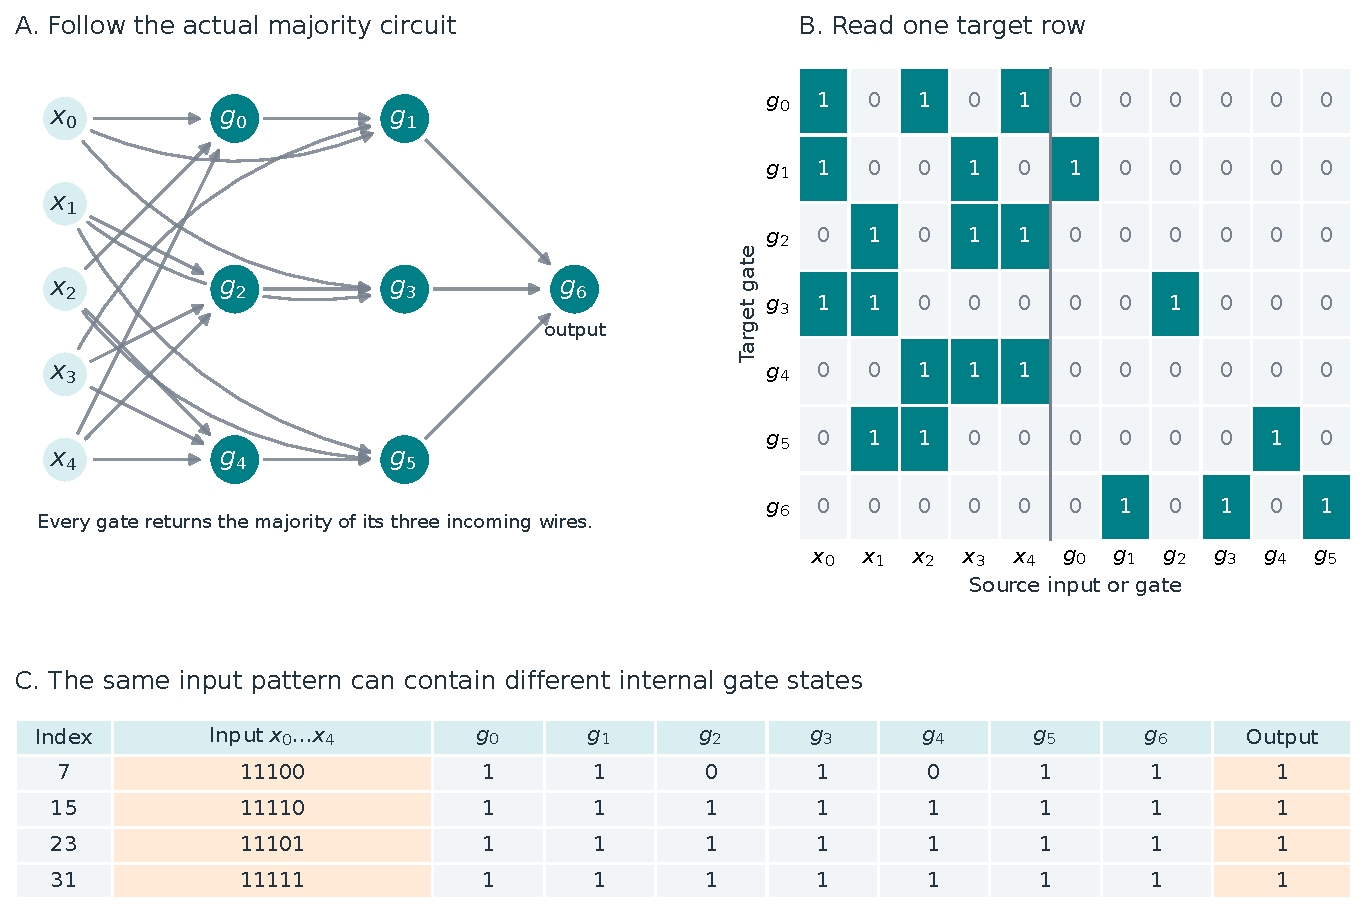
\includegraphics[width=\linewidth]{generated/majority_network.pdf}
\caption{\textbf{How does a network of small majority gates compute a larger vote?}
Panel A shows the actual five-input, seven-gate construction, with arrows
from sources to targets. Every gate computes three-input majority. Panel B
records the same connections as a matrix; each target row has three ones.
Panel C evaluates all four fillings of $111**$. Some internal outputs
change while the final output remains one. Inputs read $x_0\ldots x_4$;
their index weights are $1,2,4,8,16$.}\label{fig:network}
\end{figure}

\subsection{What index deconvolution adds}
A circuit describes how to compute an output. Its repertoire is the complete
table of outputs for all input states. Index deconvolution starts from that
table and asks which inputs actually affect the result. For a Boolean
function $f$ on $n$ bits, encode a state by
\begin{equation}\label{eq:index}
\iota(x)=\sum_{i=0}^{n-1}2^ix_i,\qquad
\mathcal I_f=\{\iota(x):f(x)=1\}.
\end{equation}
The index set $\mathcal I_f$ records exactly where the output is one; all
other indices have output zero. Input $i$ matters if there is a pair of
states differing only at $i$ for which the outputs differ. These pairs
isolate the dependence of this output condition inside the complete
repertoire. They do not imply that the integrated network or its evolving
behaviour has been reduced to a smaller table: changing the selected node
union or dynamical condition changes the observation being asked of the same
system. Equality with the original repertoire checks that the stated finite
recovery is exact.

A further compression describes groups of output-one states by patterns,
or \emph{schemata}. A schema in Holland's sense~\cite{holland1975} is a
template over $\{0,1,*\}$ in which $*$ marks a position whose value does not
affect membership, and the correspondence here is exact rather than an
analogy. Holland's $*$ is defined per template, which is why a free position
below must likewise be read per schema. Figure~\ref{fig:index} follows the
same five-input network through its ten schemata and all 32 input states.
Each schema fixes three bits to one and leaves two free. Any state with at
least three ones belongs to one or more of these patterns; no state with
fewer ones belongs to any of them.

For $111**$, the fixed ones give decimal anchor $1+2+4=7$.
The \emph{sumandos} are the fillings of the schema's don't-care positions.
Here their numerical offsets are $0,8,16,24$: set neither free bit,
only bit 3, only bit 4, or both. Adding these offsets to 7 gives indices
$7,15,23,31$, the four highlighted rows of the repertoire. The ten
schemata together expand to exactly 16 output-one indices. The union
counts each index once, even when several schemata contain it.

This anchor-and-offset reading of a schema is the representation I introduced
for estimating integrated information from algorithmic complexity and dynamic
querying~\cite{hernandez2019aid,hernandez2021aid}, where it extends Holland's
template from a device for classifying a search space into a lossless
description of a network's output repertoire: each schema is carried as its
decimal anchor together with its own family of offsets, so that queries about
the system are answered from the compressed description rather than from the
enumerated repertoire. The present response uses the same representation.

\begin{figure}[htbp]
\centering
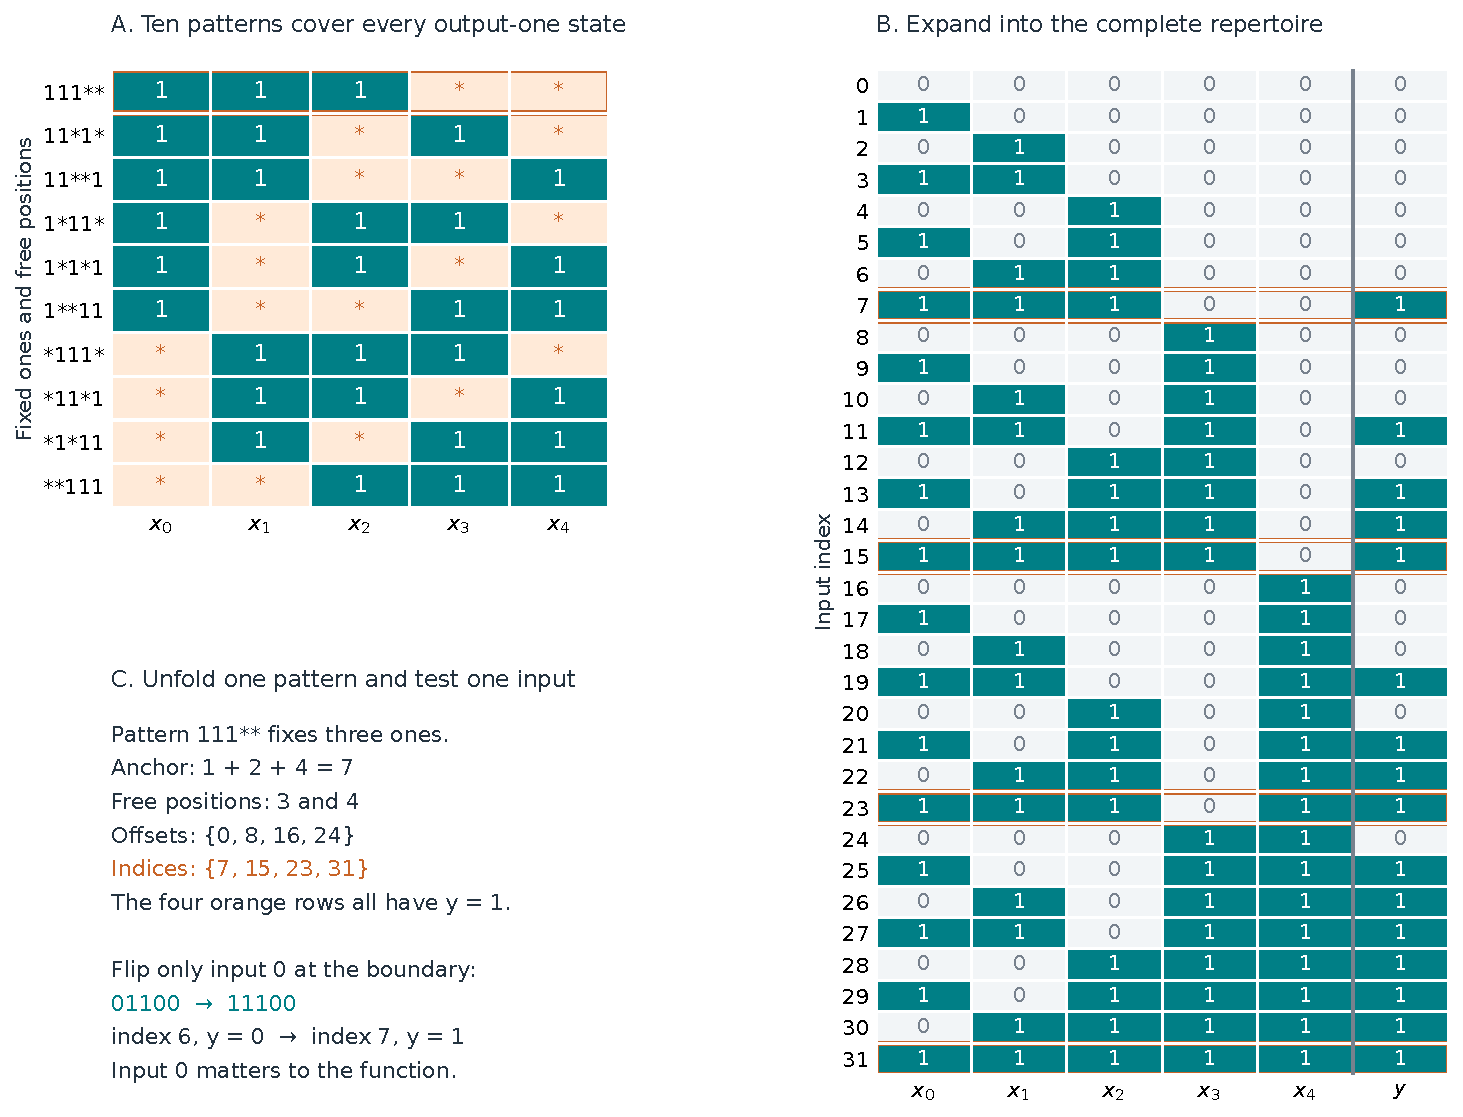
\includegraphics[width=\linewidth]{generated/majority_patterns.pdf}
\caption{\textbf{How do patterns recover the same output repertoire?}
Panel A shows the ten schemata, in Holland's sense~\cite{holland1975}, for
the network in Figure~\ref{fig:network}.
Teal entries are fixed ones; orange stars are don't-care positions, which may
be zero or one. Panel B
shows all 32 input states and the actual circuit output $y=g_6$, ordered
by input index. Orange outlines identify the four fillings of $111**$.
Panel C unfolds that pattern and shows a single-bit change that changes
the output. The figure is generated from evaluated circuit states; the
expanded schema union is checked against every output.}\label{fig:index}
\end{figure}

Free positions belong to a particular schema. In $111**$, inputs 3 and 4
can vary without changing the final answer. Both inputs still matter
elsewhere in the repertoire. For example, fixing two of the other inputs
to one makes flipping either one decisive. Likewise, changing $01100$
to $11100$ flips only input 0 and changes the output from zero to one.
These paired states are what index deconvolution uses to recover
functional dependence. The patterns and the perturbation pairs describe
two complementary aspects of the same exact map.

For odd majority on $n$ inputs, every input matters: fix the other $n-1$
bits with exactly $(n-1)/2$ ones, then flip the remaining bit. Complementation
pairs each output-one state with an output-zero state, giving $2^{n-1}$
active indices. This explains why index deconvolution does not remove
inputs from true majority, even though its output set admits schemata with
free positions.

Recovery is not limited to circuits small enough to tabulate. Run on the
decision diagram, deconvolution recovers the emitted circuit at 151 inputs:
every one of the 151 inputs comes back essential, and the recovered object is
identical to a threshold function specified by counting rather than by
majority gates. The two constructions share no code: one merges weights
recursively and emits three-input gates, the other is a dynamic program over
the coordinates. That identity settles agreement on all $2^{151}$ input states
at once, and not one of them is enumerated. Naming the recovered function is a
weaker act than recovering it, and Supplementary Section S9 says exactly how
much weaker. 

Table~\ref{tab:majority} lists the ladder, and it is worth separating its two
node columns. Recovering majority from a circuit of 8{,}116{,}950 gates
allocates 41{,}196{,}123 decision nodes, because composing the circuit gives
every intermediate wire a diagram of its own; that allocation grows as
$n^{3.96}$. The recovered function's own description is 5{,}776 nodes and grows
as $n^{1.97}$, in fact exactly $(n+1)^2/4$ at every size measured. The second
number is the one the method has to carry, and the reason it stays small is a
counting argument: read in order, the only thing a majority must remember is
how many inputs have been one so far, so a node is a position paired with a
running count. Not every function is so obliging, and
Section~\ref{sec:q8} reports one that is not. Supplementary Section S9
separates the four quantities involved, gives the per-size measurements, and
states what the comparison with the threshold specification does and does not
establish.

\begin{table}[htbp]
\centering
\caption{\textbf{Recovering majority from its own behaviour.} Each row is the
emitted circuit at that size, deconvolved and compared with a threshold
specification. Every input is recovered as essential and every comparison is an
identity, so the agreement holds on all $2^n$ states without enumerating any.
\emph{Allocated} counts every node the recovery used, most of it the diagrams of
the circuit's own intermediate wires; \emph{description} is the recovered
function's diagram alone. Supplementary Section S9 separates
them.}\label{tab:majority}
\begin{tabular}{rrrrl}
\toprule
$n$ & Gates & Allocated & Description & States covered\\\midrule
11 & 205 & 1{,}473 & 36 & $2{,}048$\\
31 & 14{,}190 & 77{,}573 & 256 & $2^{31}$\\
63 & 245{,}086 & 1{,}273{,}757 & 1{,}024 & $2^{63}$\\
101 & 1{,}623{,}175 & 8{,}304{,}498 & 2{,}601 & $2^{101}$\\
151 & 8{,}116{,}950 & 41{,}196{,}123 & 5{,}776 & $2^{151}$\\
\bottomrule
\end{tabular}
\end{table}

What is recovered is the computed function, not a unique arrangement of
internal gates. Several different circuits can share one repertoire.

Nor are an input count and an output frequency sufficient certificates.
A majority of three disjoint three-input majorities uses all nine inputs
and returns one on half its states, just like true nine-input majority.
Yet groups $110,110,000$ give local votes $1,1,0$ and an incorrect final
one: only four original bits are one. Comparing the actual index sets
exposes this failure. Supplementary Section S3 gives the reconstruction
proof, controls and limits of identifiability.
\FloatBarrier

\section{Expressing integer conditions by quadratic equations (Q5--Q8)}
These questions use a different, 254-bit prime $P$, specified in
Supplementary Section S1. Arithmetic takes place modulo $P$. A constraint
has the form $A(w)B(w)=C(w)$, where each expression is linear in the
variables $w$. A \emph{witness} is an assignment of all private and auxiliary
values satisfying the constraints.

\subsection{Designing the experiment, and what its results force}
I answered these four questions by running one experiment and then reading its
consequences, so I describe it in that order.

\paragraph{Design.} The rule I set myself was that no gate would be written
down. For each arithmetic cell I wrote only the integer relation it is supposed
to satisfy and nothing about how to compute it: $a+b+c_{\mathrm{in}}$ for the
adder, the one-bit product for the partial product, a running comparison
against a fixed bound bit for the range, and a running inequality against a
fixed constant bit for the exclusion. I then enumerated each relation's
complete behaviour over its input states, handed that behaviour to index
deconvolution, and recorded whatever came back. The method never sees a
circuit; it sees only a table of outputs.

\paragraph{Results.} The method returned, in every case, a set of inputs that
matter and a named gate acting on them. For the adder it found all three
inputs essential for both outputs and returned the sum as \textsc{xor} and the
carry as \textsc{majority}, the classical full adder, without either name being
supplied. For the one-bit product it returned \textsc{and}. For the comparison
step it returned a two-clause form on all three inputs against a bound bit of
one, and against a bound bit of zero it returned the incoming ``less'' alone,
having found the other two inputs inessential. Every recovered gate was then
folded into the gates the constraint layer carries, and each of the nine folds
was discharged by root identity rather than assumed. Figures~\ref{fig:adder-recovery}
to~\ref{fig:expansion} show these three results and the identity that licenses
the fold.

\paragraph{What the results force.} Two things are evident from what came back.
First, every object the method returned is a gate over \emph{bit} coordinates:
the essential sets it reports are sets of bit positions, and the gates it names
act on values that are zero or one. Second, the questions themselves are about
\emph{integers} --- a 64-bit bound, a canonical field element, a product of two
factors --- so the recovered network and the question do not speak about the
same objects until they are joined.

Joining them inside $\F_P$ leaves no freedom, and this is where the two
algebraic components come from. A constraint variable ranges over the whole
field, so a wire intended to carry one of the method's bits must be pinned to
$\{0,1\}$. In a single quadratic row there is exactly one way to say that:
\begin{equation}\label{eq:bit}
b(b-1)=0,
\end{equation}
the unique monic quadratic whose roots are zero and one, and which has no other
solutions because a field has no zero divisors. The compiler therefore emits
Eq.~\eqref{eq:bit} once for every input bit of every system built this way. The
integer the question asks about must then be tied to those same bits, which is
the weighted sum
\begin{equation}\label{eq:pack}
x=\sum_{i=0}^{w-1}2^i b_i .
\end{equation}
Neither equation was chosen for convenience; both are what the recovered
network needs in order to exist as field constraints at all.

\paragraph{Why the sum is an integer and not a residue.} Equation~\eqref{eq:pack}
is an identity in $\F_P$, so on its own it determines $x$ only up to a multiple
of the modulus, and a field circuit cannot distinguish $x$ from an external
$x+P$. It states what the question means only when the sum cannot wrap: with
$w$ bits the right-hand side lies in $[0,2^w-1]$, so if $2^w<P$ then that range
sits inside $[0,P-1]$ and the canonical representative of the sum equals $x$ as
an integer. This is why each width here is chosen against the modulus rather
than against the question alone --- 65 bits for Q5, 254 for Q6, 64 per factor
for Q7 --- and why the Q8 construction of Section~\ref{sec:q8} must split a
4096-bit integer into limbs instead: there no single field element can hold it,
and the bound discipline replaces Eq.~\eqref{eq:pack}.

One consequence is worth drawing out. For Q5 I take the decomposition one bit
wider than the bound, at 65 bits rather than 64. A 64-bit decomposition would
make the range true by arithmetic, since no 64-bit sum can reach $2^{64}$, and
the recovered comparator would then be verifying something it could not fail.
At 65 bits an out-of-range value is representable, and the comparator is what
rejects it. The compiled systems that result are 335 rows over 200 signals for
Q5, 2{,}193 over 1{,}223 for Q6, and 107{,}271 over 53{,}572 for Q7.

\paragraph{Two shorter relations, kept as checks.} The field can express two of
these conditions directly and far more cheaply. For $r\ne1$ one may impose
$(r-1)s=1$, which has a witness exactly when $r-1$ is invertible, and at $r=1$
would read $0=1$; for Q7 one may bound $u,v$ to 64 bits and impose $uv=n$,
which is an integer equality as well as a modular one because $uv<2^{128}<P$. I
keep both, not as the answer, but because a one-row relation that borrows the
field's own arithmetic is a useful independent check on a hundred-thousand-row
system that borrows none of it. Neither route finds factors; both verify
factors that are supplied.

\subsection{Building the same conditions out of recovered gates}
The direct equations above are short because they borrow the field's own
arithmetic. The second route asks a different question: if we are only allowed
Boolean gates, which gates are they, and who chooses them? Here nothing is
chosen by hand. Each cell is stated as an integer relation, its complete
behaviour is handed to index deconvolution, and the gate that comes back is
what gets compiled.

Handed the relation $a+b+c_{\mathrm{in}}$ and nothing else, the method returns
the sum bit as \textsc{xor} on all three inputs and the carry bit as
\textsc{majority} on all three. The classical full adder is recovered rather
than recalled. Figure~\ref{fig:adder-recovery} shows the whole of that
recovery: the eight rows the method is given, and the network it gives back.
Handed the one-bit product it returns \textsc{and}.

\begin{figure}[htbp]
\centering
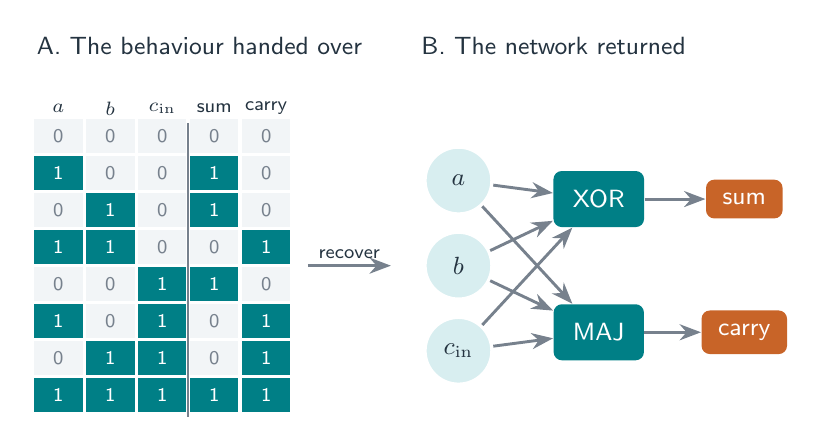
\begin{tikzpicture}[x=6.6mm,y=4.7mm]
\node[panel] at (-0.6,1.95) {A. The behaviour handed over};
\foreach \lab [count=\c from 0] in {$a$,$b$,$c_{\mathrm{in}}$,sum,carry}
  {\node[font=\sffamily\scriptsize,text=ink] at (\c,0.75) {\lab};}
\foreach \rowdata [count=\r from 0] in {{0,0,0,0,0},{1,0,0,1,0},{0,1,0,1,0},{1,1,0,0,1},%
                                        {0,0,1,1,0},{1,0,1,0,1},{0,1,1,0,1},{1,1,1,1,1}}
  {\foreach \v [count=\c from 0] in \rowdata
    {\ifnum\v=1 \node[onecell] at (\c,-\r) {1};\else \node[zerocell] at (\c,-\r) {0};\fi}}
\draw[figgrey,line width=.9pt] (2.5,0.35) -- (2.5,-7.6);
% recovery arrow between the panels
\draw[arrow] (4.8,-3.5) -- (6.4,-3.5) node[midway,above,edgelab] {recover};
% B: the returned network
\node[panel] at (6.8,1.95) {B. The network returned};
\node[innode] at (7.7,-1.2) (a) {$a$};
\node[innode] at (7.7,-3.5) (b) {$b$};
\node[innode] at (7.7,-5.8) (c) {$c_{\mathrm{in}}$};
\node[solidbox] at (10.4,-1.7) (s) {XOR};
\node[solidbox] at (10.4,-5.3) (k) {MAJ};
\node[outbox] at (13.2,-1.7) (so) {sum};
\node[outbox] at (13.2,-5.3) (ko) {carry};
\foreach \i in {a,b,c}{\draw[arrow] (\i) -- (s);\draw[arrow] (\i) -- (k);}
\draw[arrow] (s) -- (so);
\draw[arrow] (k) -- (ko);
\end{tikzpicture}
\caption{\textbf{How is the full adder recovered?} Panel A is everything the
method is given: the complete behaviour of the stated relation
$a+b+c_{\mathrm{in}}$ over its eight input states. No circuit is supplied.
Panel B is what comes back. Every one of the three inputs is found essential
for both outputs, and the two gates are named against the canonical family:
sum as \textsc{xor}, carry as \textsc{majority}. The sum is named uniquely,
while the carry's exact match class also contains \textsc{kofn} and a
two-clause regulatory form, which are the same function under other names.
These two gates, not any written by hand, are what Q7 compiles.}
\label{fig:adder-recovery}
\end{figure}

Handed a running comparison the method returns the comparator recurrence, and
once the bound bit is fixed it specialises on its own, as
Figure~\ref{fig:comparator-specialisation} shows. Against a bound bit of zero
it reports that the outgoing ``less'' depends on the incoming ``less'' alone,
because no new strict inequality can arise there. That specialisation is found,
not applied afterwards.

\begin{figure}[htbp]
\centering
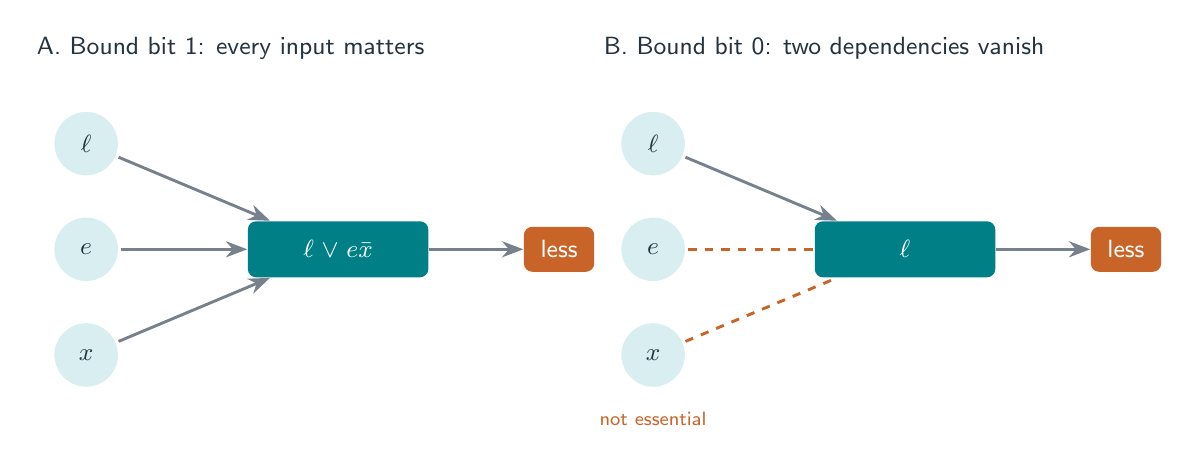
\begin{tikzpicture}[node distance=4.5mm and 15mm]
\begin{scope}
\node[panel] at (-0.75,0.95) {A. Bound bit 1: every input matters};
\node[innode] (l1) {$\ell$};
\node[innode,below=of l1] (e1) {$e$};
\node[innode,below=of e1] (x1) {$x$};
\node[solidbox,right=16mm of e1,text width=18mm] (o1) {$\ell\vee e\bar x$};
\node[outbox,right=12mm of o1] (r1) {less};
\draw[arrow] (l1) -- (o1);
\draw[arrow] (e1) -- (o1);
\draw[arrow] (x1) -- (o1);
\draw[arrow] (o1) -- (r1);
\end{scope}
\begin{scope}[xshift=72mm]
\node[panel] at (-0.75,0.95) {B. Bound bit 0: two dependencies vanish};
\node[innode] (l0) {$\ell$};
\node[innode,below=of l0] (e0) {$e$};
\node[innode,below=of e0] (x0) {$x$};
\node[solidbox,right=16mm of e0,text width=18mm] (o0) {$\ell$};
\node[outbox,right=12mm of o0] (r0) {less};
\draw[arrow] (l0) -- (o0);
\draw[cutarrow] (e0) -- (o0);
\draw[cutarrow] (x0) -- (o0);
\draw[arrow] (o0) -- (r0);
\node[edgelab,text=warm,below=2mm of x0] {not essential};
\end{scope}
\end{tikzpicture}
\caption{\textbf{The comparator specialises itself.} Both panels show the
outgoing ``less'' of one comparison step, whose inputs are the incoming
``less'' $\ell$, the incoming ``equal'' $e$, and the value bit $x$. The cell is
stated only as the meaning of a running comparison; the bound bit is a constant
of the position, and nothing else is said. Against a bound bit of one the
method finds all three inputs essential and names a two-clause form. Against a
bound bit of zero it finds $e$ and $x$ inessential and returns $\ell$ alone:
below the bound one stays below, and no zero bound bit can create a new strict
inequality. The orange dashed edges are the dependencies the method removed.
They were not removed by an optimisation pass; the cofactor test simply did not
find them.}
\label{fig:comparator-specialisation}
\end{figure}

A recovered gate names a function of any arity, while the constraint layer
carries two- and three-input gates, so the expansion between them is an
obligation rather than a convenience. It is discharged by identity for every
gate the method can return at the arities in use, and for every function of one
to three variables. Figure~\ref{fig:expansion} shows one such expansion and the
identity that discharges it.

\begin{figure}[htbp]
\centering
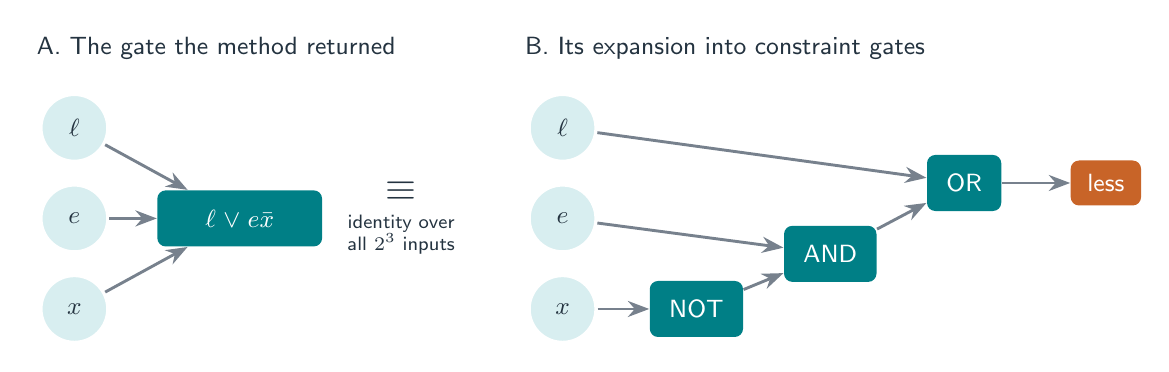
\begin{tikzpicture}
\node[panel] at (-0.6,0.75) {A. The gate the method returned};
\node[innode] at (0,0) (l) {$\ell$};
\node[innode] at (0,-1.15) (e) {$e$};
\node[innode] at (0,-2.3) (x) {$x$};
\node[solidbox,text width=16mm] at (2.1,-1.15) (g) {$\ell\vee e\bar x$};
\foreach \i in {l,e,x}{\draw[arrow] (\i) -- (g);}
% the identity that licenses the fold, drawn between the two panels
\node[edgelab,align=center,text=ink] at (4.15,-1.15)
  {\Large$\equiv$\\[2pt] \scriptsize identity over\\ \scriptsize all $2^3$ inputs};
\node[panel] at (5.6,0.75) {B. Its expansion into constraint gates};
\node[innode] at (6.2,0) (l2) {$\ell$};
\node[innode] at (6.2,-1.15) (e2) {$e$};
\node[innode] at (6.2,-2.3) (x2) {$x$};
\node[solidbox] at (7.9,-2.3) (n) {NOT};
\node[solidbox] at (9.6,-1.6) (an) {AND};
\node[solidbox] at (11.3,-0.7) (o) {OR};
\node[outbox] at (13.1,-0.7) (out) {less};
\draw[arrow] (x2) -- (n);
\draw[arrow] (n) -- (an);
\draw[arrow] (e2) -- (an);
\draw[arrow] (an) -- (o);
\draw[arrow] (l2) -- (o);
\draw[arrow] (o) -- (out);
\end{tikzpicture}
\caption{\textbf{How does a recovered gate reach the constraint layer?}
Panel A is what deconvolution returned for one comparison step: a single gate
of arity three, named as a two-clause form. The constraint layer does not carry
that gate, so it must be folded into gates the layer does carry, shown in
Panel B. The fold is not assumed correct. The expanded network is evaluated
back into a decision-diagram root, the named gate is built independently by the
engine's own gate builder, and the two roots are compared: equal roots settle
agreement on all eight inputs at once. A wrong fold cannot reach a constraint
system, because the two roots would differ and the check would fail.}
\label{fig:expansion}
\end{figure}

Q5 is the range predicate $x<2^{64}$ built from the recovered comparator, over a
decomposition one bit wider than the bound so that out-of-range values are
representable and only the comparator excludes them. Q6 uses the same
comparator at 254 bits together with a recovered inequality cell. Q7 is a
shift-and-add multiplier assembled from the recovered full adder and partial
product, at the full 64 bits the question asks for: 107{,}271 rows over
53{,}572 signals. It accepts genuine factorisations including semiprimes whose
product needs all 64 bits, and rejects trivial factors, wrong products, and a
pair of 34-bit factors whose product overflows 64 bits and would otherwise pass
as its truncated residue. Exhaustive enumeration is complete at the widths
where it is possible: every one of the 299{,}008 triples at widths four, five
and six agrees with an independent integer predicate.

This route is larger than the direct one everywhere, and no efficiency claim is
made for it. What it buys is that the gates doing the arithmetic were derived
from behaviour rather than asserted.

\begin{figure}[htbp]
\centering
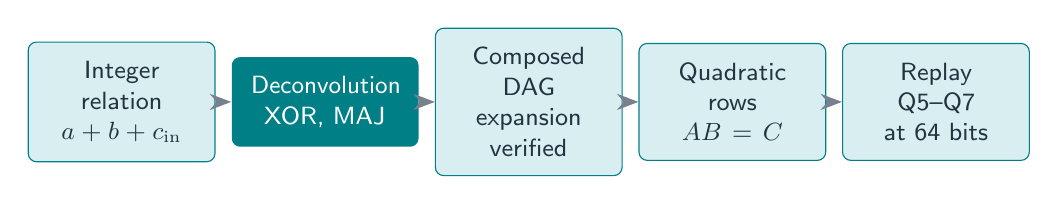
\begin{tikzpicture}[node distance=3mm and 2mm]
\node[box,text width=0.155\linewidth] (rel) {Integer relation\\$a+b+c_{\mathrm{in}}$};
\node[solidbox,text width=0.155\linewidth,right=of rel] (dec) {Deconvolution\\XOR, MAJ};
\node[box,text width=0.155\linewidth,right=of dec] (dag) {Composed DAG\\expansion verified};
\node[box,text width=0.155\linewidth,right=of dag] (rows) {Quadratic rows\\$AB=C$};
\node[box,text width=0.155\linewidth,right=of rows] (check) {Replay\\Q5--Q7 at 64 bits};
\draw[arrow] (rel) -- (dec);
\draw[arrow] (dec) -- (dag);
\draw[arrow] (dag) -- (rows);
\draw[arrow] (rows) -- (check);
\end{tikzpicture}
\caption{\textbf{From a stated relation to verified constraints.} The cell
enters as an integer relation, not as a circuit. Deconvolution names its gates,
the expansion into the constraint layer's gate set is verified by identity, and
the resulting rows are replayed against an independent predicate. No gate in
this chain is written down by hand.}
\label{fig:causalbool-route}
\end{figure}

\subsection{A large factorisation and the role of carries}
\label{sec:q8}
A 4096-bit integer exceeds the field modulus, so one field element cannot
hold it. For Q8, split each integer into 64 pieces, or \emph{limbs}, in
base $B=2^{64}$. Each limb is a 64-bit integer:
\begin{equation}
u=\sum_{i=0}^{63}u_iB^i,\qquad
v=\sum_{i=0}^{63}v_iB^i,\qquad
n=\sum_{i=0}^{63}n_iB^i.
\end{equation}
Multiply the limbs and collect terms by position, exactly as in written
multiplication. For each column $k$,
\begin{equation}\label{eq:carry}
\sum_{i+j=k}u_i v_j+c_k=n_k+Bc_{k+1}.
\end{equation}
The incoming carry is $c_k$; the outgoing carry is $c_{k+1}$. Set the
initial and final carries to zero, and set output limbs above position
63 to zero. Figure~\ref{fig:carry} illustrates how the column equations
fit together, using decimal digits so every partial product and carry
can be followed by hand. The construction above uses the same pattern
in base $2^{64}$.

\begin{figure}[htbp]
\centering
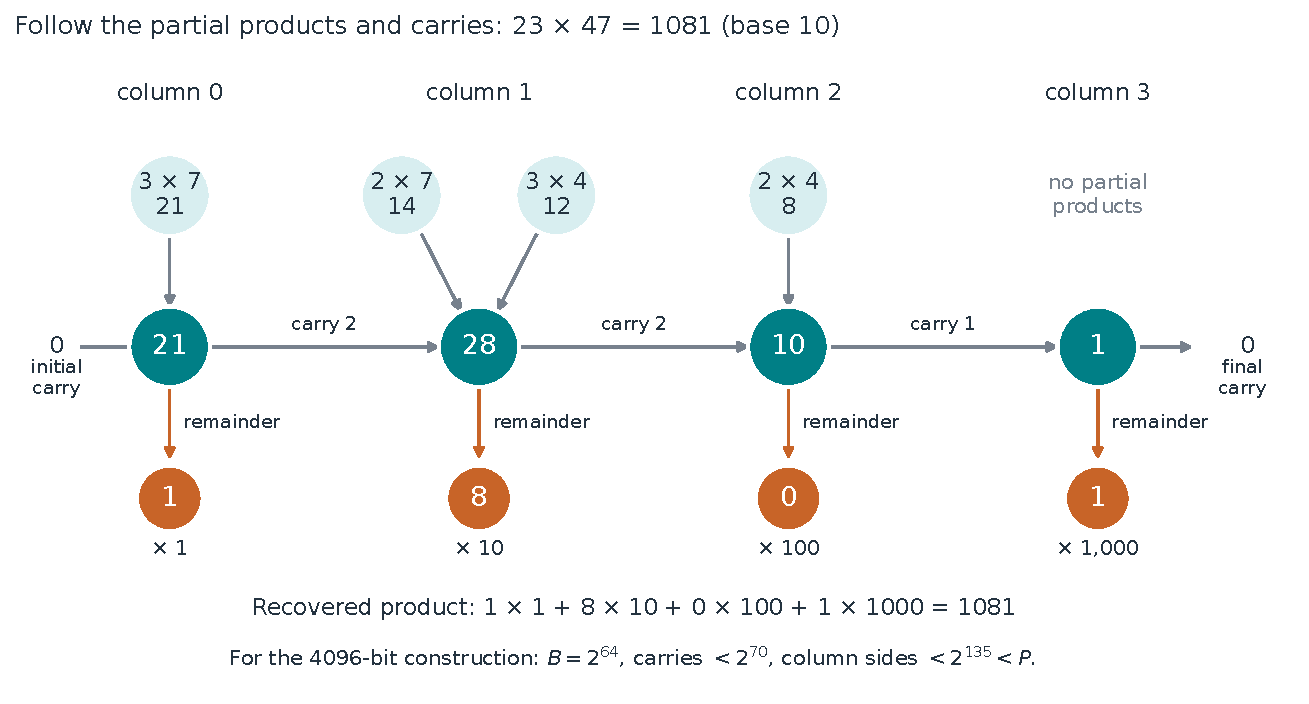
\includegraphics[width=\linewidth]{generated/carry_network.pdf}
\caption{\textbf{How do partial products become an exact integer product?}
The decimal example $23\times47=1081$ makes the carries visible. Each pale
node is a partial product. Teal nodes add the products in one column and
its incoming carry. Division by 10 sends the quotient to the next column
and keeps the orange remainder as an output digit. Columns run from least
to most significant, so the digits read $1,8,0,1$ in that order. The large
construction uses the same equations in base $2^{64}$; its limb and carry
bounds keep each column equality below the field modulus.}\label{fig:carry}
\end{figure}

The bounds are part of the argument. Intermediate carries are restricted
to 70 bits. Both sides of Eq.~\eqref{eq:carry} are then below $2^{135}<P$,
so the field cannot hide a wraparound in any column. Conversely, ordinary
multiplication produces carries within these bounds. Together with
nontrivial factors and the zero upper outputs, this proves the equivalence
between a satisfying assignment and the intended integer factorisation.

Checks evaluate these equations directly, including altered bits, partial
products, carries and public values. A useful negative control removes the
carry bounds: the false integer statement $2((P+7)/2)=7$ can then satisfy the
multiplication columns modulo $P$. Restoring the bounds rejects it.
Supplementary Sections S4--S7 give completeness and soundness proofs and the
compiled verification record.

\subsection{Where the recovered route stops, and why}
Q8 is answered above, and the recovered route of the previous subsection is not
what answers it. It is worth being precise about why, because the reason is not
effort.

The obvious attempt is to build a 4096-bit multiplier from the same recovered
cells that give Q7. Its cost follows an exact law, fitted over widths four to
sixty-four and confirmed at 128: a width-$w$ multiplier has $7w^2+1$ gates and
$26w^2+12w+7$ rows. At $w=4096$ that is 436{,}256{,}775 rows against 25{,}725
for the limb construction, a factor of about seventeen thousand. Large, but on
its own only an argument about expense.

The real obstruction appears when we ask for the compressed description rather
than the gate count. Deconvolution's reach comes from the decision diagram
staying small, and whether it does is a property of the function, not of the
implementation. Table~\ref{tab:growth} puts the two cases side by side on the
same engine. Majority's description grows polynomially, as $n^{3.96}$ across
six sizes, which is what carries it to 151 inputs. Multiplication's grows by a
factor of $2.977$ for every additional bit, measured across eleven widths, and
is already beyond a budget of eight million nodes at thirteen bits.
Extrapolating that factor to 4096 bits gives a description of some $10^{1942}$
nodes. The observable universe holds about $10^{80}$ atoms.

\begin{table}[htbp]
\centering
\caption{\textbf{Why one function is recoverable at scale and the other is
not.} Both columns are the same engine on the same machine. A majority need
only remember how many inputs are active, so its description stays polynomial.
A multiplier must retain every partial sum, and no summary suffices; the growth
is geometric and the limit is intrinsic.}\label{tab:growth}
\begin{tabular}{lrr}
\toprule
 & Majority & Multiplication\\\midrule
Description size & polynomial, $n^{3.96}$ & geometric, $\times2.977$ per bit\\
Measured over & 6 sizes, $n=31$ to $151$ & 11 widths, $w=2$ to $12$\\
Largest built & 41{,}196{,}123 nodes & 4{,}384{,}542 nodes\\
At that size & $n=151$, all $2^{151}$ states & $w=12$ bits\\
Extrapolated & --- & $\approx10^{1942}$ nodes at 4096 bits\\
\bottomrule
\end{tabular}
\end{table}

This is not a gap awaiting a better encoding. The exponential growth of such
descriptions for integer multiplication is a known lower bound~\cite{bryant},
and the measurements above are that bound appearing in our own engine. The limb
construction avoids it entirely by never going through Boolean logic: each limb
product is one field multiplication, and the blow-up has no opportunity to
occur. Reporting the boundary is more useful than omitting the question, since
it says exactly which problems this method is the right instrument for.
\FloatBarrier

\section{What this response establishes}
The solutions give a majority construction for every odd input count and
quadratic systems equivalent to the requested integer conditions. Their
assumptions determine what each answer means.

What holds these together is that one method supplies them. Index
deconvolution recovers functional dependence from behaviour and, run on a
canonical decision diagram, does so without writing the repertoire down:
majority comes back exactly at 151 inputs, and the arithmetic cells that build
Q5, Q6 and Q7 come back from stated integer relations with no gate named by
hand. The arithmetic construction then preserves integer meaning inside a
modular system by bounding every place where wraparound could occur.

The same account marks where the method does not reach. Q8 is answered by the
limb construction and not by recovery, and the reason is measured rather than
conceded: descriptions of integer multiplication grow geometrically in the
width, so at 4096 bits no such description can be written down. A method worth
using is one whose boundary is known, and this response reports both sides of
it.

The finite evidence supports these specific constructions. It includes
small majority circuits, the recovered ladder to 151 inputs and checks of
compiled arithmetic constraints. A complete 2025-input majority circuit and
generated zero-knowledge proofs remain outside that evidence. Supplementary
Information separates
the general proofs from these finite results and provides the details
needed to reproduce and assess them.
\begin{thebibliography}{9}
\bibitem{challenge} 0xPARC. \emph{Beyond Primitive Computing: Puzzles and Connections}, Field Extension.
\url{https://fieldextension.org/3b1b/}.
\bibitem{hernandez2019aid} A. Hernández-Espinosa, H. Zenil, N. A. Kiani and
J. Tegnér, \emph{Estimations of Integrated Information Based on Algorithmic
Complexity and Dynamic Querying}, arXiv:1904.10393 [q-bio.NC] (2019).
\url{https://arxiv.org/abs/1904.10393}.
\bibitem{hernandez2021aid} A. Hernández-Espinosa, H. Zenil, N. A. Kiani and
J. Tegnér, ``Estimations of Integrated Information Based on Algorithmic
Complexity and Dynamic Querying,'' in \emph{Handbook of Unconventional
Computing}, Vol. 1: Theory, ed. A. Adamatzky (World Scientific, 2021), Chap. 5,
pp. 171--220.\ \url{https://doi.org/10.1142/9789811235726_0005}.
\bibitem{holland1975} J. H. Holland, \emph{Adaptation in Natural and
Artificial Systems: An Introductory Analysis with Applications to Biology,
Control, and Artificial Intelligence} (University of Michigan Press,
Ann Arbor, MI, 1975).
\bibitem{kolmogorov1965} A. N. Kolmogorov, \emph{Three approaches to the
definition of the concept of quantity of information}, \emph{Problems of
Information Transmission} 1(1), 3--11 (1965); English reprint,
\emph{Three Approaches to the Quantitative Definition of Information},
\emph{International Journal of Computer Mathematics} 2(1--4), 157--168
(1968).\\ \url{https://doi.org/10.1080/00207166808803030}.
\bibitem{chaitin1966} G. J. Chaitin, \emph{On the length of programs for
computing finite binary sequences}, \emph{Journal of the ACM} 13(4),
547--569 (1966).\\ \url{https://doi.org/10.1145/321356.321363}.
\bibitem{li2019} M. Li and P. M. B. Vitányi, \emph{An Introduction to
Kolmogorov Complexity and Its Applications}, 4th ed., Texts in Computer
Science (Springer, Cham, 2019).\\ \url{https://doi.org/10.1007/978-3-030-11298-1}.
\bibitem{cohen} G. Cohen, I. B. Damg\aa rd, Y. Ishai, J. K\"olker,
P. B. Miltersen, R. Raz, and R. D. Rothblum.
\emph{Efficient Multiparty Protocols via Log-Depth Threshold Formulae}, 2013.
\url{https://www.wisdom.weizmann.ac.il/~/ranraz/publications/Pmajority_mpc-1.pdf}.
\bibitem{cheon} J. H. Cheon, K. Han, and M. Hhan.
\emph{Faster Homomorphic Discrete Fourier Transforms and Improved FHE
Bootstrapping}. Cryptology ePrint 2018/1073.
\url{https://eprint.iacr.org/2018/1073}.
\bibitem{causalbool} A. Hernández-Espinosa, \emph{CausalBool}, source code
accompanying this response, 2026.
\bibitem{bryant} R. E. Bryant. \emph{On the Complexity of VLSI Implementations
and Graph Representations of Boolean Functions with Application to Integer
Multiplication}. IEEE Transactions on Computers 40(2):205--213, 1991.
\bibitem{circom} iden3. \emph{Circom 2.2.3} and \emph{snarkjs 0.7.6}.
\url{https://docs.circom.io/};
\url{https://www.npmjs.com/package/snarkjs/v/0.7.6}.
\end{thebibliography}
\end{document}
